\documentclass[a4paper,11pt]{article}
%\usepackage[T1]{fontenc}

%\setlength{\textwidth}{20cm}
%\setlength{\marginparwidth}{0cm}
%\setlength{\voffset}{0cm}
\usepackage[utf8]{inputenc}
\usepackage[francais]{babel}
\usepackage{amsmath}
\usepackage{graphicx}
\usepackage{listings}
\usepackage{color}
%==== to fix locations of figures and tables
\usepackage{float}
\usepackage{placeins}

\lstset{
language=VHDL,
basicstyle=\small\sffamily,
numbers=left,
numberstyle=\tiny,
frame=tb,
columns=fullflexible,
showstringspaces=false
}
%\special{papersize=210mm,297mm}

\title{{\Huge Electronique numérique}\\Initiation à VHDL (2/3)\\Circuits séquentiels. Automates.\\ \color{red}{CORRECTIONS}}
%\title{TD1}
\date{}

\begin{document}
\maketitle

\section{Descriptions de chemin de données séquentiel}

\boxed{Questions}
\begin{enumerate}
  \item Coder en VHDL au moins deux architectures numériques qui
  réalisent un compteur, qui compte de 0 à 255, en respectant l'entité donnée ci-dessous.
  On note que les opérandes sont codés en \textbf{unsigned(7 downto 0)} (octets non-signés);
  On prendra soin de \underline{dessiner} le circuit \underline{avant} de coder l'architecture.
  \item Tester le circuit à l'aide du testbench fourni.
\end{enumerate}

\boxed{Solutions}
On présente 2 architecture, {\it in fine} identiques, mais codées différemment. L'architecture 2 semble
plus naturelle ; l'architecture 1 sépare explicitement partie combinatoire et partie séquentielle.
\begin{figure}
  \centering
  \includegraphics[width=6cm]{./compteur.png}
  \caption{Architecture du compteur, deux organisations de code possibles : soit 1 seul processus, soit 2 processus (1 processus + 1 assignation concurrente)}
  \label{compteur}
\end{figure}

\lstset{inputencoding=utf8}
\lstinputlisting[language=VHDL]{./code/compteur.vhd}

\section{Descriptions d'automates au niveau logique}
Soit un automate bien connu des informaticiens parisiens, sur la figure \ref{iloveparis}.

\begin{figure}
  \centering
  \includegraphics[width=8cm]{./iloveparis.png}
  \caption{Diagramme états-transitions de l'automate "I love Paris"}
  \label{iloveparis}
\end{figure}

\boxed{Questions}
\begin{enumerate}
  \item Vérifier que, dans le cas d'un encodage one-hot, les équations d'état suivant sont bien données par :
  $\left\{
  \begin{array}{rl}
    D_0 &= Q_0.\overline{reveil}+Q_2.\overline{bug} \\
    D_1 &= Q_0.reveil+Q_1.(greve+panne)\\
    D_2 &= Q_1.\overline{greve}.\overline{panne}+Q_2.bug\\
  \end{array}
  \right.$

  \item Coder l'automate "I\_love\_Paris" en VHDL, au niveau logique, en prenant soin de bien coder les bascules D à l'aide de processus.
  Respectez l'entité fournie ici. On utilisera une assignation conditionnelle (when) pour coder le signal de sortie "up\_and\_running".
  \lstset{inputencoding=utf8}
  \lstinputlisting[language=VHDL]{./code/i_love_paris_entity.vhd}
  %\item Ajouter un signal de sortie à votre convenance.\footnote{Sans signal de sortie, les synthétiseurs considèrent que la meilleure optimisation
  %consiste --à raison-- à générer un circuit absolument vide !}
  \item Utilisez le testbench donné sous Moodle pour tester votre automate. Observez le résultat.
\end{enumerate}

\boxed{Solutions}

\lstset{inputencoding=utf8}
\lstinputlisting[language=VHDL]{./code/i_love_paris_logic.vhd}

\section{Descriptions d'automates au niveau RTL}

Ce niveau d'abstraction RTL est le plus couramment utilisé, car il permet de
s'affranchir des détails des équations logiques, et décrire des automates (et {\it micro-architectures}) de manière plus naturelle.
Le niveau RTL repose sur la notion d'{\it inférence matérielle} : l'Electronicien doit connaître certains {\it motifs de conception}\footnote{"Design patterns", en anglais.}, afin
de permettre à l'outil de synthèse d'établir automatiquement les équations logiques sous-jacentes.
Le cas des automates d'états finis est instructif en ce sens. Voici un exemple
de codage VHDL, qui décrit un automate, sans expliciter les équations logiques sous-jacentes, ni l'encodage des états.
Pour information, le synthétiseur peut choisir de lui-même un encodage qui
maximise la fréquence de fonctionnement du circuit (encodage one-hot généralement),
ou tout autre type de contraintes imposées par le concepteur.

\paragraph{Exemple d'automate de niveau RTL}

Nous donnons ici à titre d'exemple un diagramme états-transitions, ainsi que son code VHDL de niveau RTL.
Notez que nous avons séparé le processus ici appelé "next\_state\_p", qui code
la fonction de transition (calcul de l'état suivant), et la sortie de l'automate.
\begin{center}
   \begin{minipage}[t]{8cm}
     \vspace{0pt}
     \lstset{inputencoding=utf8}
     \lstinputlisting[language=VHDL]{./code/automate.vhd}
   \end{minipage}%
   \begin{minipage}[t]{7cm}
     \vspace{40pt}
     \centering
     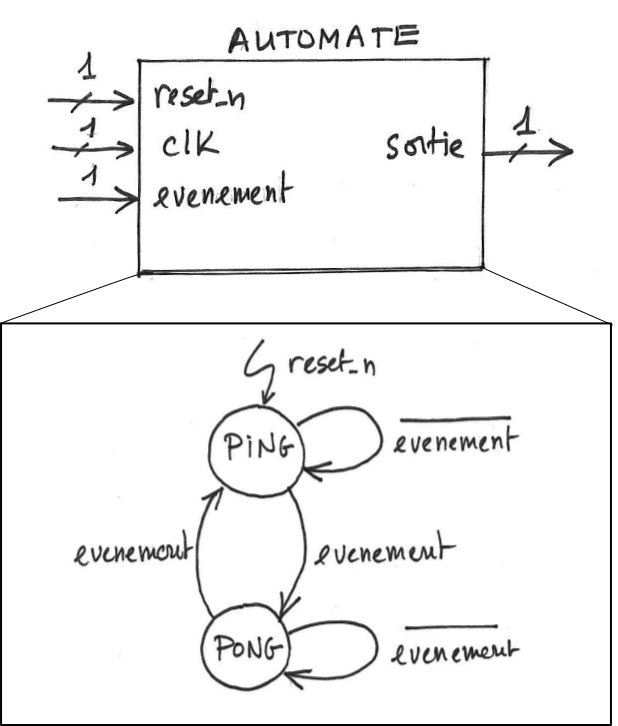
\includegraphics[width=6cm]{./ent_arch_ping_pong.png}
   \end{minipage}
\end{center} % added ending }

\boxed{Questions}
\begin{enumerate}
  \item Prenez le temps de comprendre le codage utilisé ici.
  \item Coder l'automate "I\_love\_Paris" en VHDL, au niveau RTL, en vous inspirant de l'exemple donné.
  \item Utilisez le même testbench que précédemment pour tester votre automate. Modifier uniquement le nom de l'architecture associée à l'entité instanciée.
\end{enumerate}

\boxed{Solutions}

\lstset{inputencoding=utf8}
\lstinputlisting[language=VHDL]{./code/i_love_paris.vhd}

\begin{minipage}[t]{17cm}
  \vspace{40pt}
  \includegraphics[width=16cm]{./metro_boulot_dodo_chrono.png}
\end{minipage}

\end{document}
